

\TODO{TOTAL BUDGET: 14 pages}

\TODO{TENTATIVE TARGET PAGE BUDGET: 4 pages: state of art + vision; 2 pages: methodology overview; 5 pages:
WPs; 3 pages: ethics + risks}

\tableofcontents

\newpage

\newrefsection
\chapter{B2.a State-of-the-art and objectives}

\eu{(B2.a, B2.b: max 14 pages}
\eu{

Section a: State-of-the-art and objectives. Specify the proposal objectives in
the context of the state of the art in the research field. It should be clear
how and why the proposed work is important for the field, and what impact it
will have if successful, such as how it may open up new horizons or
opportunities for science, technology or scholarship. Specify any particularly
challenging or unconventional aspects of the proposal, including multi- or
inter-disciplinary aspects.


Section B: Methodology. Describe the proposed methodology in detail including
any key intermediate goals. Explain and justify the methodology in relation to
the state of the art. Highlight any intermediate stages where results may
require adjustments to the project planning. In case you ask that team members
are engaged by another host institution, their participation has to be fully
justified by the scientific added value they bring to the project.  }

%%%%%%%%%%%%%%%%%%%%%%%%%%%%%%%%%%%%%%%%%%%%%%%%%%%%%%%%%%%%%%%%%%%%%%%%%%%
%%%%%%%%%%%%%%%%%%%%%%%%%%%%%%%%%%%%%%%%%%%%%%%%%%%%%%%%%%%%%%%%%%%%%%%%%%%
%%%%%%%%%%%%%%%%%%%%%%%%%%%%%%%%%%%%%%%%%%%%%%%%%%%%%%%%%%%%%%%%%%%%%%%%%%%
\section{A. State-of-art and objectives}

%%%%%%%%%%%%%%%%%%%%%%%%%%%%%%%%%%%%%%%%%%%%%%%%%%%%%%%%%%%%%%%%%%%%%%%%%%%
\subsection{State-of-art: social representations for intelligent robots}

Correctly interpreting our social environment is complex for machines, and has
long been identified as a key challenge on the road to competent social
robots~\cite{yang2018grand}. Accordingly, a significant, and growing, amount of
research has been dedicated to this question over the past 15
years~\cite{bartneck2020human}, without however satisfactorily coming to a
conclusion.

Let's consider the following simple illustrative example: a waiter, serving
customer in a restaurant, tell a joke. The guests look at him, smile and laugh,
and go on with ordering their dinner. As social beings, we can easily interpret
this simple description, and understand that the waiter is friendly, the guest
in a good mood, and the overall interaction is going well. Let's now consider
the same example, but the patrons do not laugh. This indicates that either the
joke was not appropriate in this context, or that the guests are not in the mood
for a joke. Either way, the interaction is not satisfactory. Finally, let
consider the same example, but this time, the waiter did not tell any joke and
was simply taking orders. Still, the guests start laughing. In this context, the
unexpected laughing tells us that something went wrong with the waiter's
behaviour.  Laughing is a relatively simple social signal to detect for a robot,
but without proper representation of the social and physical context -- and its
attached social norms -- a robot-waiter would not be able to properly understand
the situation.

To effectively interpret this situation, a robot needs a \emph{joint}
computational model of (1) the social agents relevant to the situation; (2) the
physical environment (locations and relationships between objects and other
spatial features); (3) the plans, on-going actions, and predicted results of the
tasks performed both by the robot and by the other agents; (4) a common-sense
knowledge of the social rules and norms associated to this task and context.

In addition, models for (1), (2) and (3) also have to represent \emph{dynamics} as
well: changes in the agents' behaviours, expressions, interactions; expected or
unexpected changes in the physical environment; change of plans and actions.

We review below the main approaches to build models for each of these four
aspects, as well as existing attempts to build complete models of social situations.


\subsubsection{Modelling social agents and social groups}



The importance of correctly interpreting non-verbal cues, such as facial
expressions, body language, and prosody, along with the verbal content, is well
understood in robotics as required to comprehend the emotional state and
intentions of the humans it interacts with~\cite{breazeal2003emotion}.

While the \emph{perception} of social signal has been studied in depth in the
HRI community (for instance,~\cite{pantic2011social}), and the \emph{evaluation} of
the social situation is usually handled as an aspect of the robot's decision
making, the \emph{interpretation} of social situations is a difficult problem.
It requires to build and maintain a task-appropriate model of the situations,
and represent it in such a way that a machine can reason about it.


\subsubsection{Modelling the physical context}

\subsubsection{Task modelling and action prediction}



Moreover, in a service context like a restaurant, where a robot may take on a
role similar to a waiter, misreading a social cue can lead to a breakdown in
service quality or even disrupt the customer experience. For instance, failing
to recognize a patron's displeasure with a joke might lead to repeated behavior
that further damages the relationship, whereas a socially aware robot could
adapt its interaction strategy, perhaps by offering an apology and altering its
behavior to better align with the guests' preferences~\cite{mutlu2006storytelling}.

\subsubsection{Modelling social norms}

Therefore, developing a concise representation of social situations for
autonomous social robots is crucial. Such a representation should include the
ability to model and predict the outcomes of social interactions, incorporating
an understanding of social norms, cultural context, and the potential
ramifications of deviating from expected behaviors. By doing so, social robots
can achieve a more natural and effective integration into human social spaces,
fostering positive human-robot interactions and ensuring the success of their
service functions~\cite{gockley2005designing}.


\subsubsection{Joint models of social situations}



Artificial social intelligence~\cite{bainbridge1994artificial}

researchers describe the results of social
interaction as a function not only of the individuals involved
but also of the social situation~\cite{rusbult2003interdependence}

Sociologists and social psychologists have long
recognized the importance of the situation as a determining
factor of interpersonal interaction: Atlas of Interpersonal Situations~\cite{kelley2003atlas}

Social psychologists, on the other hand, have long
considered the situation-specific aspects of interpersonal
interaction [9]. The use of social situations for examining
social interaction is widespread within both neuroscience [16]
and experimental economics [17]. Interdependence theory is a
social psychological theory developed as a means for
understanding and analyzing interpersonal situations and
interaction [9]. The term interdependence describes the extent
to which one individual of a dyad influences the other.

Wagner's \emph{outcome matrices}
\cite{wagner2006framework} \cite{wagner2009creating}

Mutual modelling:
\cite{dillenbourg2016symmetry}
stereotyping: \cite{wagner2015robots}


\TODO{copy paste from part b1}

Endsley identify in~\cite{endsley1995theory} three levels to the related concept
of \textit{situational awareness} :\emph{perception}, \emph{comprehension}, and
\emph{projection of future states}. Applied to social situation awareness,
the \emph{perception} of social signals has already been studied in depth in the
community~\cite{pantic2011social,vinciarelli2009social}.  However, relating the
resulting percepts into a comprehensive representation of a social situation
(\emph{comprehension}) and reasoning about this representation to derive an
interpretation (for instance, in terms of \emph{projections} of future social
states) are hard problems that arguably hinder further progress in social AI and
robotics~\cite{yang2018grand}. Current research is fragmented, and proposed
methods are either abstract models~\cite{gordon2016commonsense}, or task-specfic
approaches: for instance, group activity
recognition~\cite{shu2017cern,wu2019learning}; pedestrians modelling for robotic
social navigation~\cite{alahi2016social}; on-going state of an
interaction~\cite{garcía2020explainable}. We are however lacking a more
principled, general methodology to represent and reason about complex social
situations. As put by Scassellati in 2018 in the \emph{Science Robotics}' list of
ten Grand Challenges for Robotics~\cite{yang2018grand}, \emph{we have very few
comprehensive, quantitative analyses of human social responses}, and little
progress has been achieved since then.


\subsubsection{The gap in our knowledge: holistic social situations
representations}


\subsection{Embeddings as representations for social situations}

\subsubsection{Embeddings in Machine Learning}

In the context of machine learning, we refer to an \emph{embedding} as a
real-valued vector representation of a typically much higher dimensionality
input. In other words, a representation that encodes high-dimensionality input
(for instance, an image) into a lower-dimensional space. Critically, embeddings
are trained to encode the relationships and semantic nuances that might exist in
the original input space. For instance, two pictures of the same face
transformed with an embedding tuned for facial recognition would yield two
vectors that are similar to each other (i.e., close to each other for a given
metric, usually the cosine distance). As such, the process of embedding not only
condenses high-dimensional information into a more manageable form but also
captures latent associations that might otherwise remain
obscured~\cite{bengio2009learning}.

Unsurprisingly, the training of compact yet semantically-rich embeddings has
been a very active research topic over the last two decades, yielding
exceptional results in machine learning, where the (otherwise high)
dimensionality of real-world percepts might turn common machine learning
tasks like classification or prediction intractable.

While research on embeddings initially focused on data that would intuitively
lend itself well to mathematical transformations (for instance, reducing the
dimensionality of an image, represented as an array of pixel intensities, or
processing sound), it has since then been discovered that many constructs --
physical or not -- can also be \emph{embedded} in a low-dimension numerical
space, while preserving many of their semantics. One of the landmark
achievements in that regard is the work published in 2013 by Mikolov et al. --
themselves building on previous work spanning another decade.  They showed that
embeddings can be computed for \emph{words}, also encoding some of their
semantic meaning~\cite{mikolov2013efficient}, with the famous example of
\emph{embedding(`king') - embedding(`man') + embedding(`woman') $\approx$
embedding(`queen')}. Effectively, a conceptual equivalence of terms, involving
semantics related to gender and social role could be transformed into simple
mathematical additions and subtractions.

This outcome ushered in a decade of intense research on text representation,
ultimately resulting in the current Large Language Models (LLM) like GPT or
Llama2.  Most of the recent progress has been enabled by the discovery in 2017
of the attention-based \emph{Transformers}~\cite{vaswani2017attention} neural
network structure, which brought a boost to the research on natural language
procesing with, for instance, BERT~\cite{devlin2019bert} in 2019 and the family
of GPT models~\cite{wolf2020transformers} in 2020.  These large models
are pre-trained on massive text corpora and are typically used for token
prediction (the pre-trained network is fed with a text context, and predicts the
next tokens).  Importantly for this work, these very large pre-trained networks
can also be used to compute text-level embeddings, representing a short text as
a numerical vector~\cite{reimers2019sentencebert,muennighoff2022sgpt}. The
resulting embeddings can be then used to measure text-relatedness for instance,
as in the BEIR benchmark~\cite{thakur2021beir}.

\subsubsection{Social embeddings}

\begin{rewrite}
Combining the above concepts of social situations and text embeddings, we introduce in
this paper the idea of \emph{social embeddings}. A \emph{social embedding} is a
compact, real-valued numerical representation (a vector) of a social
situation, as experienced by an agent immersed in that social environment.
Following the general idea of embeddings, social embeddings are designed
to encode the \emph{semantics} of the social situation currently experienced by
the agent, facilitating the interpretation of the situation. For instance, it
could make it straightforward to compare two social situation by simply
measuring how similar the two corresponding embeddings are.

The key insight to construct these embeddings is to exploit the social knowledge
already encoded in the latent space of large language models. We do so by
automatically generating a textual description of the social environment of the
robot (using regular perception routines), and by transforming this
description into a text embedding via a large language model. By doing so, we
effectively construct an \emph{embedding}, i.e., a projection, of the social
space into a machine-friendly numerical space.

This article is a first investigation of this idea. In the following sections,
we start the exploration of the design space of social embeddings by presenting
a simple algorithm to generate scene descriptions and derive embeddings; we
analyse and discuss several key characteristics and parameters of the derived
embeddings -- like their application as a quantitative \emph{social distance};
and we discuss several promising directions for follow-up research.

\end{rewrite}

%%%%%%%%%%%%%%%%%%%%%%%%%%%%%%%%%%%%%%%%%%%%%%%%%%%%%%%%%%%%%%%%%%%%%%%%%%%
\subsection{Objectives of \project}
\label{sec:objectives}

\TODO{currently copy-paste of part B1}

\begin{rewrite}

\noindent At the basic research level, \project targets two overarching research goals:

\begin{enumerate}[label=\textbf{(\arabic*)}]
    \item to build compact, yet semantics-preserving, embeddings to represent
arbitrary social situations; and to fully characterize these embeddings,
including their latent semantics. I translate this first goal into objective
{\bf O1}:

\begin{enumerate}[label=\textbf{O\arabic*}]
    \item \label{O1} To \textbf{construct and characterize the fundamental
properties of social embeddings}.
\end{enumerate}

    \item to precisely \textbf{define and implement the socio-cognitive skill of
        \emph{social situation awareness} enabled by social embeddings}. I split this
        second goal into three specific objectives: \emph{social appraisal},
        \emph{social prediction}, \emph{social learning}.

\begin{enumerate}[label=\textbf{O2.\arabic*}]
    \item \label{O2.1} To use social embeddings to \textbf{automatically appraise
        social situations}, taking into account their \textbf{context}. Using
        a set of prototypical reference situations~\cite{kelley2003atlas}, social embeddings
        can be used to relate the current social situation to known ones.
        Besides, because social embeddings lend themselves to jointly encode
        social context by simply attaching context descriptions, the appraisal
        of the social situation can be made \emph{context-aware};

    \item \label{O2.2} To use social embeddings to model \textbf{social
        dynamics} by characterizing the trajectories of on-going social situations in the
        embedding space. I will look in particular into trajectories'
        \emph{discontinuties}, that might represent unexpected changes of social
        dynamics, and trajectories' \emph{extrapolations}, that might represent
        \textbf{social situation \emph{predictions}}.

    \item \label{O2.3} To \textbf{learn socially-appropriate behaviours} by using
        social embeddings as an additional input feature to existing robot behaviour
        generation algorithms, and by augmenting existing interactive machine
        learning techniques (`user in-the-loop' social learning for robots, that I
        pioneered in e.g.~\cite{winkle2021leador}) with
        representations of the social situation;

\end{enumerate}
\end{enumerate}

\noindent To illustrate these objectives, let consider the following imaginary
scenario: a robot is welcoming visitors at the entrance of an hospital; a group
of 3 persons are discussing together; one person is standing in the middle of
the room, glancing around; one last person is entering the hospital and
walks toward the reception. \ref{O2.1} will show that social embeddings can
represent and appraise this situation, accounting for the `hospital entrance' context: while
the person walking towards the reception probably does not need help from the
robot, the one in the middle seems uncertain, and might appreciate a pro-active
helping behaviour from the robot. \ref{O2.2} adds the temporal dimension: if we
sample the scene at regular time steps, and build a sequence of social
embeddings, what trajectory do they follow in the embedding space? Is it
continuous? Is there any rapid changes? Can we extrapolate this trajectory to
predict where the situation is going? \ref{O2.3}, finally, looks at exploiting
social embeddings for socially-aware behaviour learning. In our scenario, a
member of the hospital staff would for instance teach the robot an
context-appropriate response, and the robot would be able to generalise it to
other, similar social situations.


I want to evidence these properties in both lab-based experiments and
real-world deployments on social robots. Accordingly, \project has two addtional
objectives:

\begin{enumerate}[label=\textbf{O\arabic*}]
    \setcounter{enumi}{2}
    \item \label{O3} To fully {\bf integrate social embeddings onto a
        socio-cognitive architecture for autonomous service robots} and,

    \item \label{O4} To conduct an {\bf ambitious experimental programme},
        including both lab-based and field research, to demonstrate the
        effectiveness of social embeddings in complex, real world conditions.
        This means deploying the \project robot into existing social eco-systems
        that are sufficiently complex, yet open to explore novel social interactions.
\end{enumerate}


\end{rewrite}

\subsubsection{Basic research objectives}

\subsubsection{Empirical research objectives}


%%%%%%%%%%%%%%%%%%%%%%%%%%%%%%%%%%%%%%%%%%%%%%%%%%%%%%%%%%%%%%%%%%%%%%%%%%%
\subsection{Importance and impact of the project}

\begin{rewrite}

Academically, the \project project represents a timely combination of
very recent advances in supervised machine learning for social robot
behaviour with a creative and interdisciplinary approach to the design
and automation of social robot behaviour. 
We will publish \project results in interdisciplinary and high-profile
discipline-specific journals (eg. Science Robotics; Frontiers in AI and
Robotics; Transaction in Human-Robot Interaction) and conferences (eg. AAAI,
HRI, RSS).

The dataset of social behaviours and social signals we will create and
distribute represents a one-in-a-kind resource for the human robot
interaction community, and the human data collection will be
transferable to research in other domains such as human-computer
interaction.

As \project will be deployed in a living lab environment, there is
significant scope for public outreach/engagement and media coverage,
which we will work with the BRL's media manager to maximise.


\project aims at building unique European capacity to assert leadership in this
domain, and, beyond the specific deliverables of this 5-years project,
establishing the PI as a world-leader in goal-driven, socially-responsible
robotics.

\end{rewrite}

%%%%%%%%%%%%%%%%%%%%%%%%%%%%%%%%%%%%%%%%%%%%%%%%%%%%%%%%%%%%%%%%%%%%%%%%%%%
\subsection{Interdiscplinary nature of the project}

My project aims at introducing a completely new approach to the represention of
social situations. While \project focuses on embodied artificial social agents
like social robots, the basic research that I will conduct (WP1 and WP2) is
essentially independent of the domain of application, and might impact the whole
subfield of digital humanities related to the study of our social world.

Accordingly, the project is grounded in both the psycho-social literature of
human cognition, and the latest technological advances in artificial cognition
and human-robot interaction, and aims at delivering major conceptual, technical
and experimental contributions across several fields: intelligent robotics,
machine learning and AI, data-driven social psychology and sociology, ethics. By
working at the crossroad of these discipline, \textbf{\project builds bridges
across multiple disciplinary boundaries}.

\project delivers this programme using a range of scientific methods,
previously outlined in Part B1, combining for instance machine learning and
embedding-based data representation, with non-verbal social perception and field
observations of social behaviours.

Accordingly, the project builds on a \textbf{strong interdisciplinary team}: the
post-docs directly recruited on \project will have backgrounds in deep machine
learning (PD1) data-driven sociology (PD2, PHD1), cognitive modeling (PD3),
cognitive robotics (PHD2). Additional expertise will be recruited to provide
specific support: Dr. Maribel Pino and the Broca hospital living lab will
contribute their expertise on robot deployment and study orgnisation in an
hospital environment; the \project Ethics Advisory Board will contribute
expertise to guide the work on ethics.

%%%%%%%%%%%%%%%%%%%%%%%%%%%%%%%%%%%%%%%%%%%%%%%%%%%%%%%%%%%%%%%%%%%%%%%%%%%
%%%%%%%%%%%%%%%%%%%%%%%%%%%%%%%%%%%%%%%%%%%%%%%%%%%%%%%%%%%%%%%%%%%%%%%%%%%
%%%%%%%%%%%%%%%%%%%%%%%%%%%%%%%%%%%%%%%%%%%%%%%%%%%%%%%%%%%%%%%%%%%%%%%%%%%
\newpage
\section{B. Methodology}

%%%%%%%%%%%%%%%%%%%%%%%%%%%%%%%%%%%%%%%%%%%%%%%%%%%%%%%%%%%%%%%%%%%%%%%%%%%
\subsection{Overview of \project methodology}

\subsubsection{Research methodologies}

As presented in the Part B1, \project combines multiple scientific
methodologies to achieve the four objectives listed in
Section~\ref{sec:objectives}.



\subsubsection{Implementation of the work program}

I organise the project in four work-packages, aligned with the four objectives
(Figure~\ref{fig:wps}): \textbf{WP1} is dedicated to the construction and
characterization of social embeddings; \textbf{WP2} exploits social embeddings
to develop a new form of artifical social situation awareness; \textbf{WP3} looks at how
social robots can make use of this skill by integrating social embeddings into
existing cognitive architectures for service robots; and \textbf{WP4} organises
the experimental work, both lab-based and in-the-wild, that demonstrates the
\project approach in ambitious and complementary situations.


\begin{figure}[h!]
\centering
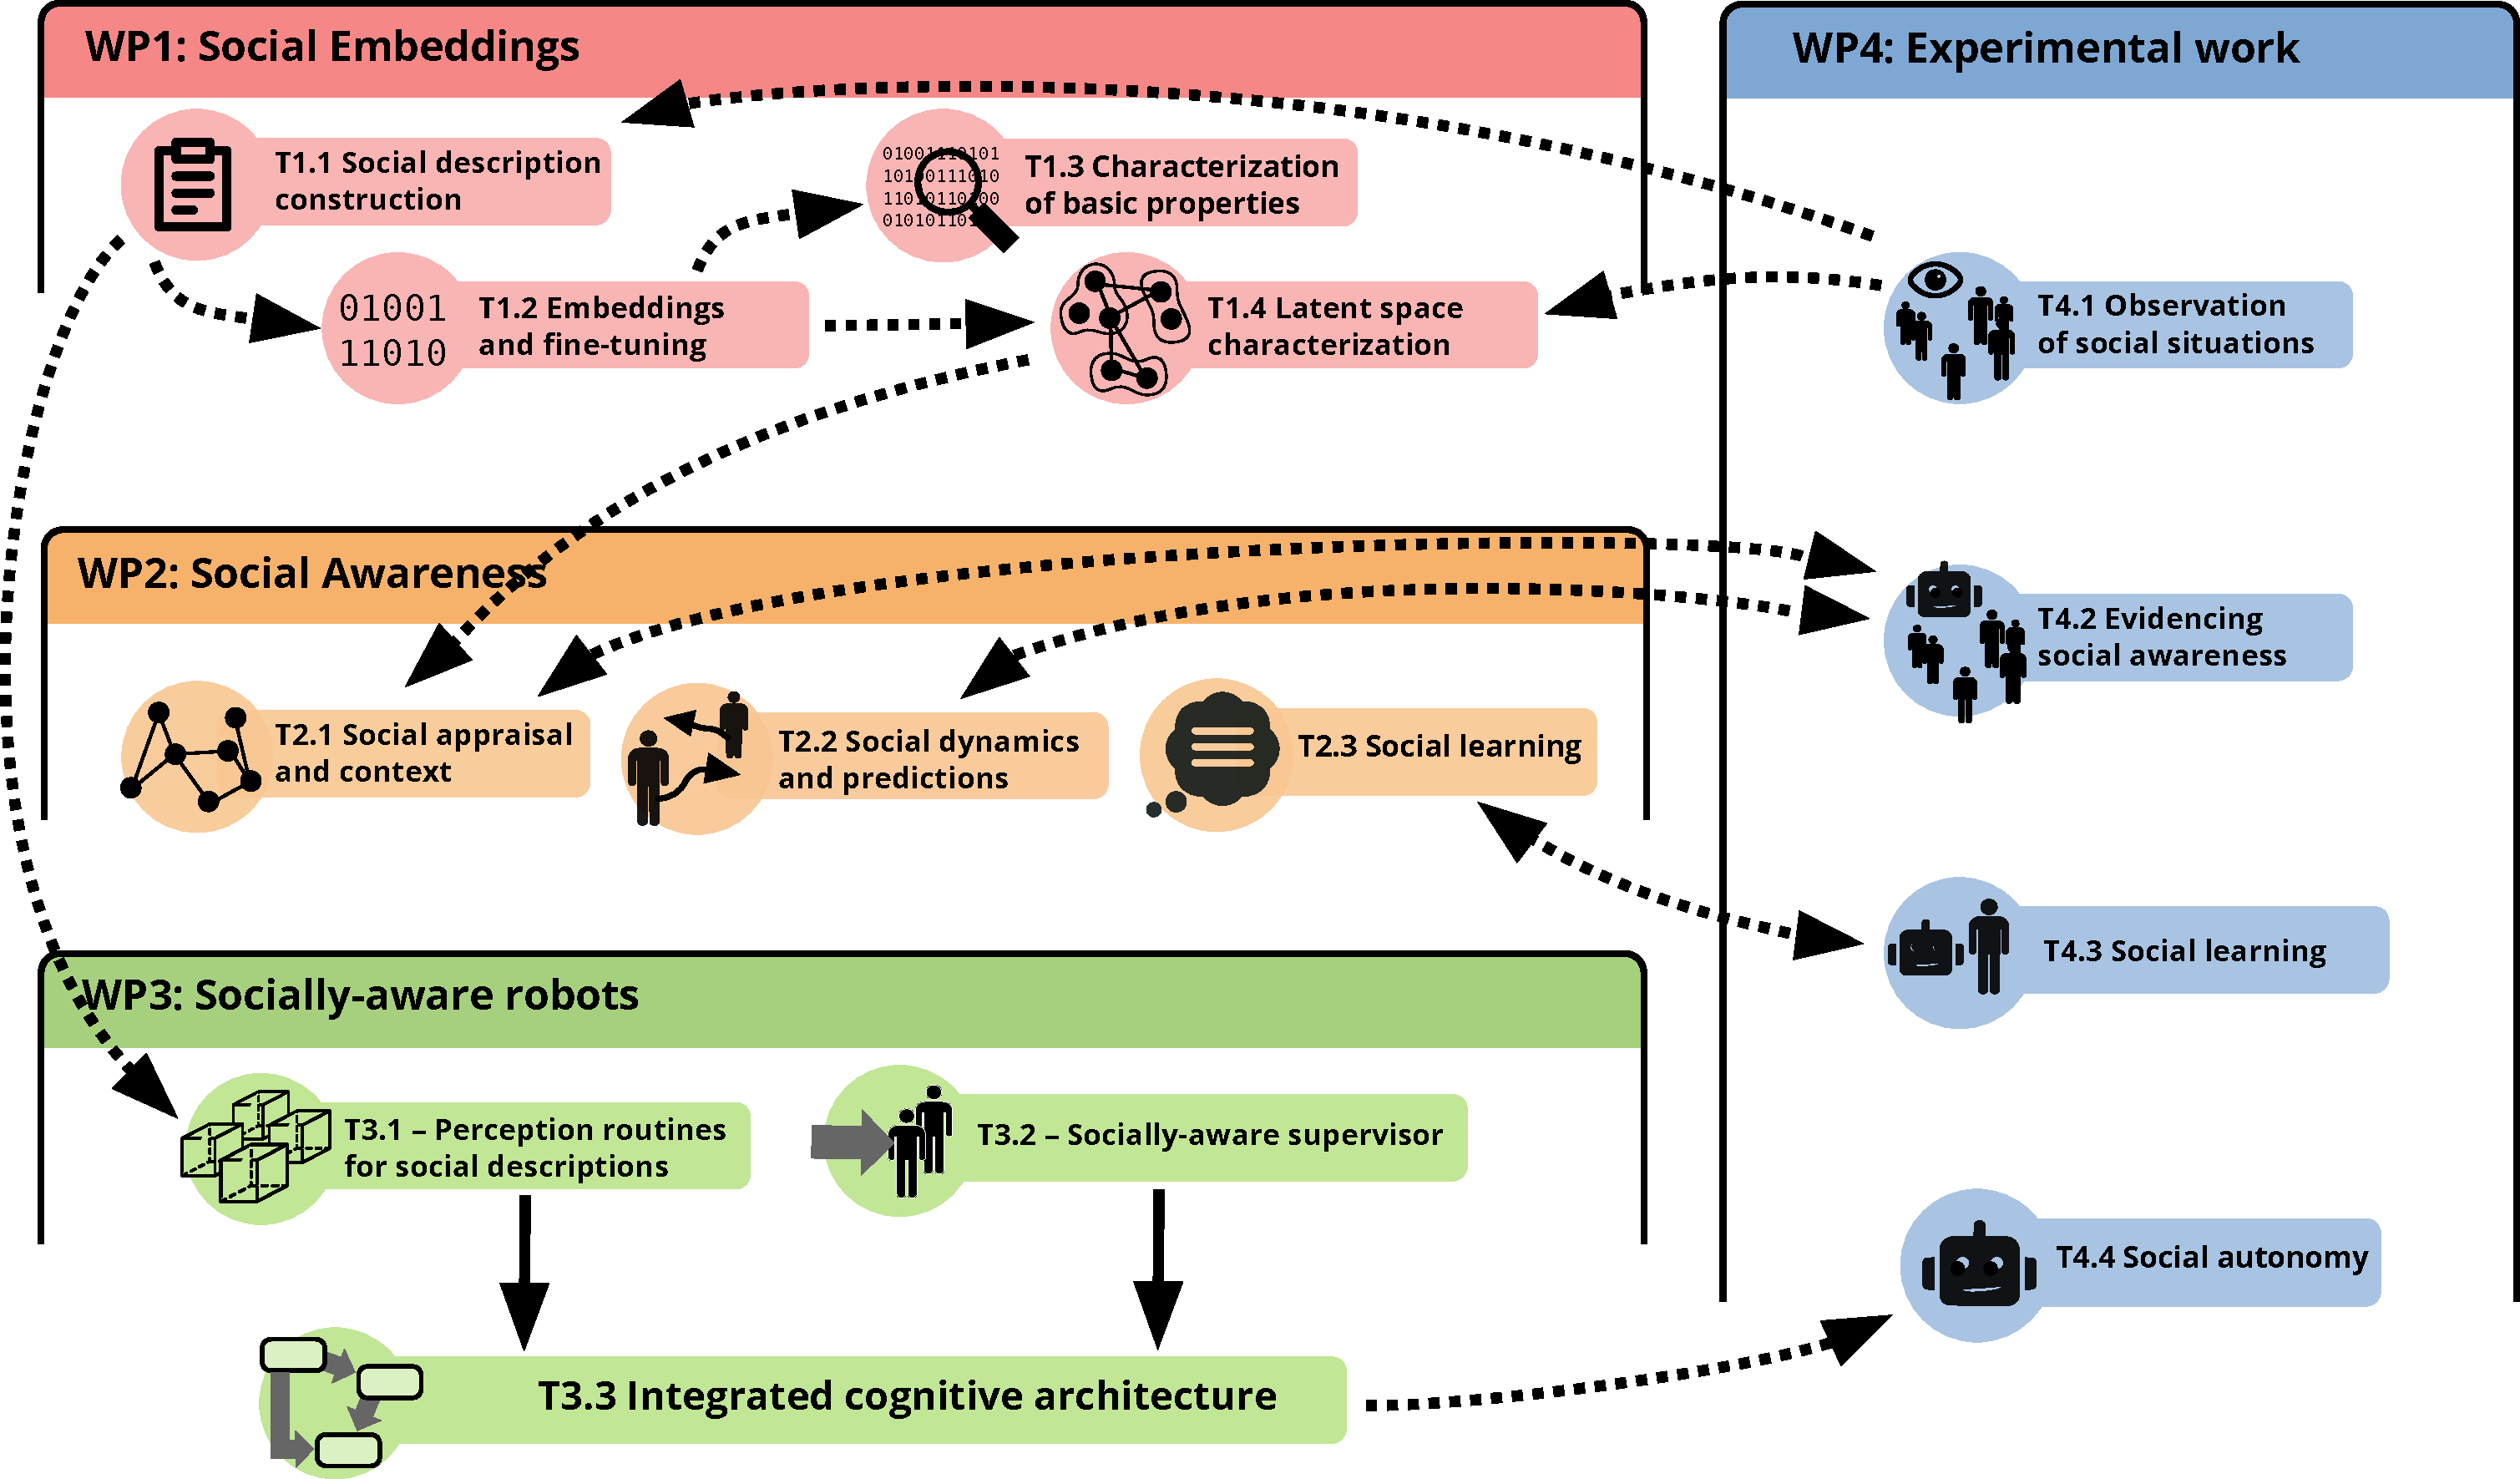
\includegraphics[height=0.6\linewidth]{figs/wps}
\caption{Overview of the workpackages and tasks, and tasks inter-relations.}
\label{fig:wps}
\end{figure}

More specifically, Figure~\ref{fig:wps} gives an overview of the project
workpackages, and their interrelations.


\subsubsection{Social Robotics as an experimental framework}

As a \emph{methodology} to represent and reason about social situations, social
embeddings are fundamentally agnostic from their final domain of application.
However, the practical study and validation of social embeddings does require
experimental grounding through artificial social agents embedded into
complex-enough social situations. In \project, I choose to exploit social robots
as an experimental platform.  Beyond my extensive experience and know-how in
social robotics, both at the basic level and at the experimental level, several
scientific and practical reasons drive this choice.

First, compared to many other AI systems (e.g. virtual avatars), robots
are physically situated.  They can partake to a broad range of naturalistic
social situations and social interactions, providing means to acquire,
fine-tune, and validate social embeddings in a variety of real-world scenarios.

Second, not only robots are physically situated, but they also have access to a rich
range of sensing modalities for social perception (including vision, audition).
Combined with robots' proprioception and localisation capabilities, these
percepts can be fully spatially-grounded. This let us compute a rich set of
social constructs (for instance, mutual gaze or joint attention), that feed
directly into the available social descriptors.

Third, social robots are \emph{active} social agents. From an experimental point
of view, robots' behaviours can be
designed to induce and influence specific social situations, providing us with a
invaluable tool to study social situations and related sociodynamics.

Finally, beyond the suitability of social robotics as an experimental
methodology for the \project project, the field of social robotics in itself is
``hitting a wall''~\cite{yang2018grand} in trying to build appropriate tools to represent and
reason about the social environment of robots. By specifically applying social
embeddings to social robotics, I also aim to provide new, groundbreaking
tools to the robotic community to build more intelligent social robots.

\subsubsection{Gantt chart}

%\begin{landscape}
\begin{figure}[!h]
\resizebox{\linewidth}{!}{
    %%%%%%%%%%%%%%%%%
%%
%% Task dependencies
%%
%% Task...        depends on Task...
%% T1.3           T1.1
%% T1.3           T1.2
%% T1.2           T2.2 (user interface)
%% T3.3           T2.3
%%

\definecolor{barcolor}{RGB}{153,204,254}
\definecolor{linkred}{RGB}{165,0,33}
%\renewcommand\sfdefault{phv}
%\renewcommand\mddefault{mc}
%\renewcommand\bfdefault{bc}
\setganttlinklabel{s-s}{START-TO-START}
\setganttlinklabel{f-s}{}
\setganttlinklabel{f-f}{FINISH-TO-FINISH}

%\begin{sidewaysfigure}[!ht]
\begin{figure}[!ht]

%\sffamily
\begin{ganttchart}[
        canvas/.append style={fill=none, draw=black!5, line width=.75pt},
        hgrid style/.style={draw=black!5, line width=.75pt},
        vgrid={*1{draw=black!5, line width=.75pt}},
        %vgrid={*1{black}, *{11}{black!5}}, % doesnt work for some reason
        x unit=.35cm,
        y unit chart=.65cm,
        time slot format=isodate-yearmonth,
        time slot unit=month, % pgfgantt >= 5.0
        %compress calendar, % pgfgantt < 5.0 => overleaf
        title/.style={draw=none, fill=none},
        title label font=\bfseries\footnotesize,
        %title label node/.append style={below=7pt},
        include title in canvas=false,
        bar label font=\mdseries\small\color{black!70},
        %bar label node/.append style={left=2cm},
        bar/.append style={draw=none, fill=barcolor!50},
        bar progress label font=\mdseries\footnotesize\color{black!70},
        group/.append style={fill=barcolor},
        group incomplete/.append style={fill=black},
        group left shift=0,
        group right shift=0,
        group height=.5,
        group peaks tip position=0,
        group label node/.append style={left=.6cm},
        group progress label font=\bfseries\small,
        link/.style={-latex, line width=1.5pt, linkred},
        link label font=\scriptsize\bfseries,
        link label node/.append style={below left=-2pt and 0pt,
        milestone/.append style={circle},
        milestone inline label node/.append style={left=5mm}}
    ]{2021-01}{2025-12}
    
        %\gantttitle[
        %    title label node/.append style={below left=7pt and -3pt}
        %]{Month:\quad1}{1}
        \gantttitlecalendar{year, month} \\
        %\gantttitlelist{0,5,...,60}{1} \\
        %% WP1
        \ganttgroup[]{WP1 \wpOneShort}{2021-01}{2023-12} \\
            \ganttbar[name=WP11]{\textbf{1.1} Conceptual framing \& ethics}{2021-01}{2023-12} \\
            \ganttbar[name=WP12prep,inline,bar/.append style={fill=gray!20}]{preparation}{2021-07}{2021-12}
            \ganttbar[name=WP12exp,inline]{WeTheCurious experiment}{2022-01}{2022-12}
            \ganttbar[name=WP12]{\textbf{1.2} Principles of r-HHI}{2023-01}{2023-06} \\

        %\ganttlink[link type=f-s]{WBS1A}{WBS1B}

        %% WP2
        \definecolor{barcolor}{RGB}{153,2,254}
        \ganttgroup[]{WP2 \wpTwoShort}{2021-01}{2024-12} \\
            \ganttbar[name=WP21]{\textbf{2.1} Situation assessment}{2021-01}{2022-06} \\
            \ganttbar[name=WP22]{\textbf{2.2} Social dynamics}{2022-01}{2023-12} \\
            \ganttbar[name=WP23]{\textbf{2.3} Group dynamics}{2024-01}{2024-12} \\
            \ganttbar[name=WP24]{\textbf{2.4} Social situation assessment}{2022-07}{2024-12} \\

        %\ganttlink[link type=f-s]{WP21}{WP24}
        %\ganttlink[link type=f-s]{WP22}{WP23}

        %% WP3
        \definecolor{barcolor}{RGB}{50,220,134}
        \ganttgroup[]{WP3 \wpThreeShort}{2021-01}{2025-12} \\
            \ganttbar[name=WP31]{\textbf{3.1} Social teleology}{2023-01}{2024-12} \\
            \ganttbar[name=WP32]{\textbf{3.2} Human-in-the-loop policy learning}{2021-07}{2025-06} \\
            \ganttbar[name=WP33]{\textbf{3.3} Integrated cognitive architecture}{2021-01}{2025-06} \\

        %\ganttlink[link type=f-s]{WP12}{WP32}

        %% WP4
        \definecolor{barcolor}{RGB}{244,50,20}
        \ganttgroup[]{WP4 \wpFourShort}{2022-01}{2025-12} \\
            \ganttbar[name=WP41]{\textbf{4.1} Behaviours baselining}{2022-01}{2022-12} \\
            \ganttbar[name=WP42]{\textbf{4.2} Generative behaviours}{2023-01}{2023-12} \\
            \ganttbar[name=WP43]{\textbf{4.3} Non-verbal behaviours}{2023-07}{2025-12} \\


        %% WP5
        \definecolor{barcolor}{RGB}{234,200,20}
        \ganttgroup[]{WP5 \wpFiveShort}{2022-07}{2025-12} \\
            \ganttbar[name=WP51prep,inline,bar/.append style={fill=gray!20}]{preparation}{2022-07}{2022-12}
            \ganttbar[name=WP51]{\textbf{5.1} SEN schools experiment}{2023-01}{2023-12} 
            \ganttbar[name=WP51expl,inline,bar/.append style={fill=gray!20}]{analysis}{2024-01}{2024-06} \\
            \ganttbar[name=WP52prep,inline,bar/.append style={fill=gray!20}]{preparation}{2024-01}{2024-06}
            \ganttbar[name=WP52]{\textbf{5.2} children hospital experiment}{2024-07}{2025-06}
            \ganttbar[name=WP52expl,inline,bar/.append style={fill=gray!20}]{analysis}{2025-07}{2025-12} \\

        %\ganttlink[link type=f-s]{WP41}{WP51}


        %\ganttlink[link type=f-s]{WBS1B}{WBS1C}
        %\ganttlink[link type=f-f,link label node/.append style=left]{WBS1C}{WBS1D}

        \ganttmilestone{\bf\sc Integration sprints}{2021-06}
        \ganttmilestone[milestone/.append style={fill=orange, circle}]{}{2021-11}
        \ganttmilestone{}{2022-06}
        \ganttmilestone[milestone/.append style={fill=orange, circle}]{}{2022-11}
        \ganttmilestone{}{2023-06}
        \ganttmilestone{}{2023-12}
        \ganttmilestone[milestone/.append style={fill=orange, circle}]{}{2024-05}
        \ganttmilestone{}{2024-12}


        % separate years
        \ganttvrule[vrule/.append style={gray, dotted, thin}]{}{2021-12}
        \ganttvrule[vrule/.append style={gray, dotted, thin}]{}{2022-12}
        \ganttvrule[vrule/.append style={gray, dotted, thin}]{}{2023-12}
        \ganttvrule[vrule/.append style={gray, dotted, thin}]{}{2024-12}


        \ganttvrule{start @WeTheCurious}{2021-12}
        \ganttvrule{start @SEN school}{2022-12}
        \ganttvrule{start @Children hospital}{2024-06}

\end{ganttchart}

%\end{sidewaysfigure}
\end{figure}

}
\label{gantt}
\end{figure}
%\end{landscape}


\subsubsection{Project's milestones}

\begin{table}[h!]
    \centering
\begin{tabular}{@{}lccccccr@{}}
\toprule
\textit{\textbf{}}              & \textbf{Y1} & \textbf{Y2} & \textbf{Y3} & \textbf{Y4} & \textbf{Y5} \\ \midrule
\textit{MS1:...} &   & x  &    &   &    &  &   \\ 
\textit{MS2:...} &   &    & x  &   &    &  &   \\ 
\textit{MS3:...} &   &    &    & x &    &  &   \\ 
\textit{MS4:...} &   &    &    &   & x  &  &   \\ \bottomrule
\end{tabular}
    \caption{Project's milestones}
    \label{milestones}
\end{table}

\subsubsection{Additional methodological measures}

\paragraph{Integration sprints}

\project is a complex project, with numerous interdependencies between tasks.
To ensure the interdependencies are properly understood, and support effective
integration of the outputs of each workpackage, I will organise every 6 months,
and for the first 4 years, \textbf{integration sprints} (see Gantt diagram).
Integration sprints are one-week long integration retreats during which the whole
\project team gather and work together to effectively implement and test on the
robot the different components. In addition to providing regular `check points'
for the project, they also set a stable schedule to deliver project components.

This methodology was used by the PI in  several previous projects (FP7 CHRIS
project, H2020 SPRING for instance), and had proved to be of great value to
ensure project-wide cohesion and steady progress.

\paragraph{Software engineering and open-access}

The project will follow strict software engineering guidelines, based on the
experience I gained while working in the industry, with specific measures to
ensure the public access and long-term archival of the artifacts produced during
the project. In particular:

\begin{itemize}
    \item code development will exclusively take place on a public code versioning
        platform (e.g. GitHub), under a permissive open-source license (Apache
        2.0);
    \item where relevant, code will be systematically accompanied of
        documentation, unit-tests, and easy-to-run examples;
    \item I will make use of the Continuous Integration and Continuous
        Deployment (CI/CD) capabilities of the code platform to automatically
        run code linting and unit-tests before merging code to the repository's
        main branch;
    \item robot-specific code will be developed using the ROS 2 standard,
        ensuring a high degree of compatibility with other projects;
    \item the integration of the robot architecture (\tCC) will be based on individual Dockerized
        components for each of the robot's capabilities, continuously integrated
        and tested via \texttt{docker compose} and dedicated integration tests;
    \item the project's code repositories and artifacts (e.g. fine-tuned models)
        will be indexed and synchronized on EU-compatible long-term archival
        repositories like Zenodo.  
\end{itemize}

%%%%%%%%%%%%%%%%%%%%%%%%%%%%%%%%%%%%%%%%%%%%%%%%%%%%%%%%%%%%%%%%%%%%%%%%%%%
\subsection{Expertise and Research team}
\label{research-team}

My expertise is primarily centered on cognitive robotics and human-robot social
interaction. My expertise in this field covers a broad spectrum, from basic
research in robotics (for
instance~\cite{lemaignan2014dynamics,lemaignan2015mutual}) and data-driven
socio-psychology
(including~\cite{lemaignan2014cognitive,irfan2018social,winkle2019effective,bartlett2019what}),
to technical contributions (for instance~\cite{lemaignan2010oro,
lemaignan2017artificial, lemaignan2018underworlds}), to extensive experimental
work (see below; for instance~\cite{hood2015cowriter,winkle2020couch,
lemaignan2022social}).

Over the last 4 years, I have re-focalised my work on \emph{data-driven HRI},
contributing several new large datasets of social
interactions~\cite{lemaignan2018pinsoro,sallami2020unexpected,webb2023sogrin},
developing new data analysis
techniques~\cite{bartlett2019what,webb2022measuring}, and demonstrating with my
students new applications of interactive machine learning to social
interactions~\cite{senft2016sparc,winkle2020couch,winkle2021leador}.  In
parallel, I progressively matured the idea of computing compact
\emph{embeddings} of social situations, until I recently published a first
breakthrough in that direction~\cite{lemaignan2024social} (to appear at IEEE/ACM
HRI'24). This ERC project is directly born from this multi-year endeavour
towards data-driven social sciences applied to embodied AI systems, and aims at
significantly accelerate research in this direction.

In particular, \project is the opportunity to gather an interdisciplinary team
of academics that would effectively complement my expertise, and ensure the
feasibility of the project.

Specifically, I intend to recruit:

\begin{itemize}

    \item  two researchers with expertise in data-driven
        socio-psychology (one senior post-doc PD1, one PhD student PHD1); these
        researchers will directly contribute to the human data acquisition,
        the interpretation of social embeddings in term of social situations,
        and the experimental work;

    \item two researchers with expertise in deep machine learning and large
        language models (one senior post-doc PD2, one PhD student PHD2); these
        researchers will contribute to the core implementation of social
        embeddings, including language model fine-tuning, as well as the
        analysis of the embedding space topology;

    \item one research in cognitive robotics (PhD student, PHD3); this
        researcher will focus on the effective integration of social
        embeddings into a larger cognitive architecture for social robots, able
        to autonomously drive interactions;

    \item one researcher in ethics of technology (post-doc
        level PD3); this researcher will lead the work on understanding social
        embeddings in terms of ethical and responsible research.
\end{itemize}

Table~\ref{time-allocation-team} provides an overview of the time allocation per
members of the team, over the course of the project.

\begin{table}[h!]
    \centering
\begin{tabular}{@{}lccccccr@{}}
\toprule
\textit{\textbf{}}              & \textbf{Y1} & \textbf{Y2} & \textbf{Y3} & \textbf{Y4} & \textbf{Y5} &  & \textbf{Total months} \\ \midrule
\textit{Séverin Lemaignan (PI)} & 1         & 1         & 1         & 1
    & 1         &  & 60                    \\ \midrule
\textit{Post-doc 1 (WP1)}       & 1           & 1           & 1           &             &             &  & 36                    \\
\textit{Post-doc 2 (WP2)}       & 1           & 1           & 1           & 1           &             &  & 48                    \\
\textit{Post-doc 3 (WP3)}       &             & 1           & 1           & 1           & 1           &  & 48                    \\
\textit{Post-doc 4 (WP3, WP5)}  & 1           & 1           & 1           & 1           & 1           &  & 60                    \\
\textit{PhD 1 (WP3, WP5)}       &             & 1           & 1           & 1           & 0.5         &  & 42                    \\ \bottomrule
\end{tabular}
    \caption{Full-time equivalent for the research team members\TODO{to update}}
    \label{time-allocation-team}
\end{table}


In addition, the host institution (INRIA Grenoble) will provide extensive
additional expertise on machine learning applied to robotics. I will specifically build on
my already established collaboration with Dr. Xavier Almeida-Pineda, head of the
RobotLearn research group. Dr. Almeida-Pineda is the coordinator of the EU H2020
SPRING project on social robotics for geriatric care, on which I collaborated
for the past two years.

Additional expertise, as well as access to one of my main experimental
environment, will be provided through a collaboration with Paris' public
hospitals (APHP) and specifically, with Dr. Maribel Pino, head of research at
Paris' Broca geriatrics hospital (Dr. Pino has extensive experience running
studies with social robots on the hospital' premisses).


%%%%%%%%%%%%%%%%%%%%%%%%%%%%%%%%%%%%%%%%%%%%%%%%%%%%%%%%%%%%%%%%%%%%%%%%%%%
\subsection{Workpackages}

\subsubsection{WP1: \textbf{\WPA}}

WP1 addresses Objective \textbf{O1}. I will first systematically investigate the
three steps of social embeddings construction, and then characterize the
resulting embeddings.


\paragraph{\TAA}

Social embeddings construction requires first to extract descriptors, then to
build complete textual descriptions, and finally to embed these descriptions.  I
will extract basic social descriptors using the ROS4HRI social perception
approach, as it formalize a multi-modal model of humans~\cite{lemaignan2022ros},
and run in real-time on current robots. I will augment these basic descriptors
with more complex percepts, including (1) descriptors of human-objects
interactions (HOI), using transformer-based techniques
like~\cite{iftekhar2022what} ; (2) affective
descriptors~\cite{vinciarelli2009social}, using e.g. facial expressions based on
facial action units classification~\cite{martinez2019automatic}; (3) group-level
interactions, including $f$-formations~\cite{setti2015fformation}, and group
activity recognition, using deep convolutional graph techniques like
ARG~\cite{wu2019learning}.

%(3) a novel contextual model of
%attention~\cite{ferrini2024percepts} that allows fine-grained assessment of what
%the person around the robot are focusing on.

The generation of textual descriptions consists in both the combination of
descriptors into textual \emph{snapshots} of the social environment at a
specific time, and the combination of these snapshots over time, to build a
textual description of complete situations with a time horizon of 10s to
25s~\cite{netanyahu2021phase}. I will initially build snapshots using text
templates, and then extend the methodology using techniques based on
social knowledge graphs~\cite{sap2019atomic} and propositional
logic~\cite{tsoi2022sean}. The combination of snapshots into social situations
will be developed with the help of the PHASE simulator and
dataset~\cite{netanyahu2021phase}, that includes a large number of annotated
social interaction sequences.

\begin{framed}
    {\noindent\bf Main outcomes of \tAA:} lorem ipsum 
\end{framed}

\paragraph{\TAB}

This task focuses on the text embedding process itself. Due to the fast pace of
progress in the LLMs landscape, it is likely that current methods (including
e.g.~\cite{reimers2019sentencebert,muennighoff2022sgpt}) will have been
superseeded by new methods. I will closely monitor advances in the domain,
especially on the question of semantic relatedness~\cite{thakur2021beir}, as
this is critical for social embeddings. I plan to also perform
fine-tuning~\cite{hadsell2006dimensionality} of the selected text embedders to
specialize them for social situation representation. I will do so by leveraging
existing open-access annotated datasets of social interaction like
AMI~\cite{carletta2007ami}, D64~\cite{oertel2013d64},
SALSA~\cite{alameda2015salsa}, or my own SoGrIn dataset~\cite{webb2023sogrin},
and datasets of social questions-answers like SocialIQa~\cite{sap2019social}.

\begin{framed}
    {\noindent\bf Main outcomes of \tAB:} lorem ipsum 
\end{framed}

    \paragraph{\TAC}

\begin{rewrite}
I will then characterise social embeddings, starting with the fundamental
properties that I identified in~\cite{lemaignan2024social}: invariance to
syntax, social similarity and continuity. 
\end{rewrite}

\begin{framed}
    {\noindent\bf Main outcomes of \tAC:} lorem ipsum 
\end{framed}

\paragraph{\TAD}

\TODO{rephrase; be more specific (eg cf Sun's paper)}

This task will look into the characterization of the embeddings' \emph{latent
semantics}: For instance, social descriptions like `two persons chatting and
laughing together'; or `a group of three people walking together'; or `one
single person walking towards the robot, looking agitated'; etc.  are all
semantically distinct, and, consequently, would belong to distinct regions in
the embedding space. Identifying such clusters to characterize the semantic
topology of the embedding space~\cite{sun2023topological} will be achieved by
exploiting existing annotated datasets to identify and extract prototypical
reference social situations.

\begin{framed}
    {\noindent\bf Main outcomes of \tAD:} lorem ipsum 
\end{framed}


\begin{framed}
    \noindent{\bf WP Timeframe:} Y1-Y3.5; one post-doc ({\bf PD1}) with expertise in
    deep learning/text embedding; one post-doc ({\bf PD2}) in data-driven
    sociology.
\end{framed}

\subsubsection{WP2: \textbf{\WPB}}

\emph{Social situation awareness} is a socio-cognitive skill that is essential for
artificial social system, like social robots, to e.g.  act in a
context-sensitive manner, reason and apply social norms, or create proactive
social agents (in order to acknowledge and respond to a human who would like
to engage with the robot, the robot must first adequately model and
recognise the corresponding social situation).

Work package WP2 focuses on research objectives \ref{O2.1}, \ref{O2.3} and \ref{O2.2}:
expanding social embeddings beyond their fundamental properties, to build a
`social situation awareness' cognitive skill for social robots.

\TODO{justify these 3 objectives}
\begin{itemize}
    \item appraise social situations, also taking into account the social context
    \item learn socially-appropriate behaviours
    \item anticipate future social states
\end{itemize}



\paragraph{\TBA}

The first task of this workpackage focuses on \emph{social appraisal}.

Social appraisal (Objective~\ref{O2.1}) is about interpreting the results of WP1
in terms of social situations\TODO{...}

Context-awareness is another critical aspect of social situation appraisal.
\emph{Context} has been defined in various way, including as \emph{who},
\emph{what}, \emph{when}, \emph{where}, and \emph{why} of
interactions~\cite{vinciarelli2009social}; as high-level task/environment
characteristics, such as `studying' or `dining'~\cite{nigam2015social}; as
relationships between agents in the scene, such as `interacting in a group',
`standing in a line'~\cite{althaus2004navigation}; or as
task-based~\cite{castellano2012detecting}. Social embeddings lend themselves
well to context encoding: as long as a context description can be generated, it
can be appended to the social situation description, and jointly embedded.
I will use \TODO{list context sources + algos: location, robot's role, on-going
task, etc}
%
%\emph{Characterizing} how context impacts the resulting social embeddings
%requires extensive research, from defining and specifying a taxonomy of
%contexts, to characterizing their impact on the social embedding space.

\TODO{need to be SMART: reference specific techniques + metrics}

This task is linked to the experimental task \TDB.


\begin{framed}
    {\noindent\bf Main outcomes of \tBA:} lorem ipsum 
\end{framed}

\paragraph{\TBB}

This task looks onto how social embeddings can offer a novel approach to the
modelling and interpretation of \emph{social dynamics}. I hypothesise that
social dynamics correspond to \emph{trajectories} of social situations in the
embedding space.  For instance, the velocity in the embedding space should
reflect the rate of change of a social situation in the physical space;
trajectory extrapolation could be employed by robots to anticipate upcoming
social situations; discontinuities in the embedding space would reflect brutal
social changes that could trigger specific robot behaviours (for instance to
acknowledge or attempt to repair social situations).  \TODO{need to be SMART:
reference specific techniques + metrics}


\begin{framed}
    {\noindent\bf Main outcomes of \tBC:} lorem ipsum 
\end{framed}

\paragraph{\TBC}

Objective~\ref{O2.3} and the learning of socially-appropriate behaviour
generation, \project aims at significantly advancing the state of the art in
this regard, by combining two techniques: (1) generative neural networks
for affective robot motion
generation~\cite{marmpena2019generating,suguitan2020moveae}; (2) interactive
machine learning in high-dimensional input/output spaces, where I have shown
with my students promising results for generating complex social
behaviours~\cite{senft2019teaching, winkle2020couch} that fully involve the
end-users~\cite{winkle2018social}. Modulating (1) with the social embedding of
the current situation will enable the generation of non-repetitive and socially
appropriate behaviours (gestures, motions, gazing behaviours, facial
expressions); augmenting the input space of (2) with social embeddings will
enable the robot to learn contextualised social policies

This task is linked to the experimental task \tDD.

\begin{framed}
    {\noindent\bf Main outcomes of \tBB:} lorem ipsum 
\end{framed}


\begin{framed}
    \noindent{\bf WP Timeframe:} Y2-Y4; one post-doc ({\bf PD3}) in cognitive
    sciences; one PhD student in data-driven sociology ({\bf PHD1}).
\end{framed}





\subsubsection{WP3: \textbf{\WPC}}

\begin{rewrite}

WP3 design and implement on the TIAGoPro robot the principled cognitive architecture
that binds together the socio-cognitive perceptual capabilities of the robot
(WP2), with its action production mechanisms (WP3).

\textbf{T3.1 -- A social teleology for robots}
\emph{Teleological systems} (ie goal-driven) has been investigated in robotics
for being a way of providing long-term drives to an autonomous robot. This has
been successfully applied to curiosity-driven robots~\cite{oudeyer2005playground} or motor babbling in infant-like
robots~\cite{forestier2017unified}, but only for relatively simple cognitive
systems. This task's objective is to define and implement a novel \emph{social teleology} that would
algorithmically encode long-term social goals into the robot. This will directly
build from the results of WP1, where interaction principles for social robots
are experimentally uncovered.

\begin{framed}
    {\noindent\bf Main outcomes of T3.1:} the algorithmic translation of WP1's
    interaction principles in long-term social goals for the robot, eg a
    long-term, socially-driven action policy for the robot.
\end{framed}

\textbf{T3.2 -- Learning from humans to achieve `by-design' responsible \&
trustworthy AI}
Building on my recent, promising results on human-in-the-loop
social learning~\cite{senft2019teaching,winkle2020couch}, this task
implements the learning mechanics (including the bi-directional interface
between the human teacher and the robot) to allow human end-users to
teach the robot domain-specific (at school, at the hospital) social policies,
following the methodology and the interactive reinforcement learning approach I
developed with my students in~\cite{senft2017supervised}.

In addition, this task will study through qualitative methods (thematic
interviews and questionnaires) how human-in-the-loop machine learning enables a more
trustworthy AI system, by involving the end-users in the creation of the robot
behaviours, thus offering a level of behavioural transparency to the end-users.

\begin{framed}
    {\noindent\bf Main outcomes of T3.2:} a human-in-the-loop reinforcement
    learning paradigm, suitable for in-situ teaching of the robot by the
    end-users themselves.
\end{framed}

\textbf{T3.3 -- Integrating a socially-driven architecture for long-term interaction}
This task builds on the state of art in cognitive architectures (disembodied
ones~\cite{chong2007integrated,vernon2007survey,kingdon2008review,duch2008cognitive,langley2009cognitive,taatgen2010past,thorisson2012cognitive},
as well as ones specifically developed for robotics:
ACT-R/E~\cite{trafton2013act}, HAMMER~\cite{demiris2006hierarchical}, PEIS
Ecology~\cite{saffiotti2005peis,daoutis2012cooperative},
CRAM/KnowRob~\cite{beetz2010cram, tenorth2009knowrob},
KeJia~\cite{chen2010developing}, POETICON++~\cite{antunes2016human}, and my own,
the LAAS Architecture for Social Interaction~\cite{lemaignan2017artificial}):
the overall purpose of the socio-cognitive architecture of \project is to
integrate in a principled way the spatio-temporal and social knowledge of the
robot (WP2) with a decision-making mechanism, to eventually produce
socially-suitable actions (WP3). 

The decision-making mechanism is the heart of the \project AI engine: the robot
will rely on it to generate action decision that are purposeful, legible and engaging on the
long run, something that none of the existing architectures have been able to
successfully demonstrate to date. I aim at a breakthrough, and will
introduce a novel approach: drawing from the interaction patterns identified
in T1.2, I will combine long-term, socially-driven goals (\emph{social teleology}, T3.1), and
human-in-the-loop machine learning (T3.2) using a novel arbitration mechanism.

to make ensure local adaptation  progressively learn an social
policy enabling long-term autonomy. This task focuses on `bringing the pieces
together' in a principled manner.


The arbitration mechanism itself will build on research on reinforcement
learning for experience transfer~\cite{madden2004transfer} that enables the
re-assessement of a policy (here, our long-term social teleology) based on
specific experience (here, the end-user-taught policy).


\begin{framed}
    {\noindent\bf Main outcomes of T3.3:} A cognitive architecture, implemented
    on the TIAGoPro robot, that enables long-term social engagement, by combining
    long-term goals with domain-specific action policies, taught by the
    end-users themselves.
\end{framed}

\end{rewrite}


\paragraph{\TCA}

lorem ipsum

\begin{framed}
    {\noindent\bf Main outcomes of \tCA:} lorem ipsum 
\end{framed}

\paragraph{\TCB}

lorem ipsum

\begin{framed}
    {\noindent\bf Main outcomes of \tCB:} lorem ipsum 
\end{framed}

\paragraph{\TCC}

lorem ipsum

\begin{framed}
    {\noindent\bf Main outcomes of \tCC:} lorem ipsum 
\end{framed}


\begin{framed}
    \noindent{\bf WP Timeframe:} Y1.5-Y4; one ... ({\bf PDx}) with expertise in
    ...; one ... ({\bf PDx}) in ...
\end{framed}











\subsubsection{WP4: \textbf{\WPD}}


\begin{rewrite}

\project has the ambition to demonstrate long-term, co-designed social
interactions in two complex, socially sensitive spaces.
The first one involves the deployment of social robots in special needs schools
(SEN schools) in Bristol (O2.1.1). Building on a rigorous participatory approach
involving the school teachers, as well as the parents, we will seek to integrate
the robot in the daily life of the school, supporting the development of the
students' physical and social skills. The second one takes place in Bristol's
Children's Hospital (O2.1.2), supporting isolated children who suffer long-term
conditions, in close cooperation with the hospital staff. In both cases, a
social robot will be deployed on premises, for one un-interrupted year. It will
integrate the daily routines of the institutions, under supervised
autonomy~\cite{senft2017supervised}, and \emph{without} requiring the
presence of a researcher at all time.

These two experiments raise specific practical and ethical questions, as they
target vulnerable populations. This is an however informed choice: first, I
already have established partnerships with Bristol's children hospital on one
hand, and a network of Bristol-based SEN schools on the other hand. As such, and
from a practical perspective, I do not foresee any institutional issues -- on
the contrary, our partners are excited at the prospect of taking part to the
project. Besides, convincingly demonstrating the importance and positive impact
of socially-driven, socially-responsible robotics does accordingly require
complex social situations, and complex social dynamics. The two scenarios, which
complement each other, provide both. These scenarios also put the project in the
unique position of actually delivering high societal impact: we anticipate 30+
hospitalised children with long-term conditions, and 250+ SEN-educated children
to directly benefit of the project, showing how robots can have a lasting,
beneficial impact on the society, alongside human carers: it will establish the
idea of \emph{robots supporting human interactions} instead of dehumanising our
social relationships.

Both these deployments will take place within the strict ethical framework
established in T1.1, the ethical considerations pertaining to these experiments
are further discussed below, in the section on ethics, and in the separate annex
on ethics, uploaded alongside this proposal.


\TODO{explain that these 2 large experiments will be scaffolded by many smaller
ones}

\textbf{O2.1.1: A robot companion to support physical, mental and social
well-being in SEN schools}

Inspired by a similar large-scale deployment of social robots in Hong-Kong's SEN
schools~\cite{robot4sen}, the first study investigate whether a socially
assistive robot can effectively support the development, social
interactions and well-being of children with a long-term mental condition. This
study will take place within the network of Bristol-based SEN schools, with
which I already have an on-going collaboration.  Specifically, the two main
questions we seek to investigate are: What are the social underpinnings of the
successful integration of a social robot in the school ecosystem? Can ambitious
co-design with the end-users (teachers) deliver a `net gain' for the learning,
social interaction and well-being of the students? 

The core of the study consists in deploying the R1 social robot in one of
Bristol-based SEN school (Mendip Primary School, with possible extensions to
other schools), to investigate how the robot can help shaping a social school
ecology that fosters mental well-being, while effectively supporting teachers
and students in their learning. 

The study will adopt a strong participatory design approach, inspired by
Patient and Public Involvement methodologies (PPI~\cite{boivin2010patient}),
with 3 one-day focus groups organised with the school teachers; two evening focus group with the
school parents, prior to the study; and several preparatory workshop at the
school premises to involve the students as well.

%During the first
%workshop, the teachers will be introduced to the robot capabilities with
%examples of robot-supported teaching activities, and the robot's visual
%programming interface will be introduced. We will also conduct group discussions
%on how the robot can best be integrated in the daily school routine and
%classroom context. During the second workshop, the teachers will be invited to
%create novel activities, with the support of the research team. An evening focus
%group will be organised as well with the parents, to integrate their
%perspectives in the design of the robotic system.  Will we formally analyse the
%data from this – will it become a research paper? 

%Following the workshops, the teacher-oriented codesign of the robot's activities
%and supervision tools (eg to start/stop/pause/resume activities) will be
%finalised and implemented by the research team.

The school study itself will take place during Y3, with the robot permanently
based at the school. The robot will take part in the
regular teaching and other daily routines of the school, and will directly
interact with the children, learning its action policy (`when to do what') from
initial co-design with the teachers, followed by progressive in-situ teaching (see
O2.3.2).

During selected `observation days', observations will be conducted by the
research team, and regular semi-structured interviews will be conducted with the
teachers, parents, and where possible, the children themselves (using engagement
metrics like the Inclusion of Other in Self task and Social-Relational
Interviews~\cite{westlund2017measuring}), to understand how the robot impacts
the school dynamics  (both positively and potentially negatively).

The task will be jointly supervised with local colleague and expert Dr.Nigel Newbutt,
who has a long track record of working with special needs schools.

\textbf{O2.1.2 -- A robot companion to support isolated children during their
hospital stay}

The second experiment will take place within the paediatric ward for long-term
conditions at the Bristol Children's Hospital. The ward has 8 beds, with
children staying from a few weeks to several years. Over the course of the
one-year deployment, we expect the robot to interact with about 30 children,
their parents, and the hospital staff (nurses, doctors).

Similar to the first experiment, we will be using a \emph{mutual shaping}
approach~\cite{winkle2018social} to design the role of the robot with the
different stakeholders (nurses, doctors, parents, children), in order to
experimentally investigate how a social robot can support hospitalised children
with long-term conditions. The robot's role will revolve around facilitating
social interactions between (possibly socially isolated) children, by fostering
playful interaction within the paediatric ward.

This second experiment complements the first one by evidencing the commonalities
and divergences in terms of social interactions when the robot is moved to a
different environment. While the hospital eco-system is comparatively smaller that the SEN school one,
people `live' at the ward day and night; it becomes \emph{de facto} the second home of the
children, and the children will have more interaction opportunities than at the
SEN school (where the robot is shared amongst a larger group). As a consequence,
we expect to observe different interaction patterns, with potentially deeper
affective engagement between the robot and the other ward's `inhabitants'.
Specific safeguarding measures will be put in place with the hospital team, and
resulting observations will feed into the ethical guidelines of T1.1.

\end{rewrite}


\paragraph{\TDA}

The social situation awareness capabilities enabled by the use of social embedding will be
demonstrated through the following studies:

\begin{itemize}
    \item {\bf situational awareness (SA)}: instead of relying on the standard
        SAGAT test~\cite{endsley2017direct}, I will use a protocol proposed by
        Dahn et al. in~\cite{dahn2018situation}, specifically designed for
        robots, and based on the ability for a robot to recognised an event as
        being unexpected. This protocol ha the advantage of being directly
        adaptable to social embeddings.

    \item {\bf social intelligence quotient (SQ)}, for instance, the George Washington University Social Intelligence Test~\cite{moss1930social}
\end{itemize}

\begin{framed}
    {\noindent\bf Main outcomes of \tDA:} lorem ipsum 
\end{framed}

\paragraph{\TDB}

I will adapt to social
robotics~\cite{lemaignan2015mutual} experimental protocols originally designed
by Frith and Happé~\cite{frith1994autism} to investigate social representation
and mental modelling in autistic children.  This protocol include tasks like
distinguishing \emph{happiness} or \emph{sadness} from \emph{surprise}, or
distinguishing \emph{sabotage} from \emph{deception}: these nuances, quite
self-explanatory to experienced social agents, require subtle modelling of the
context and mental state of agents, and, until now, have not been successfully
reproduced on robots. I aim to show that social embeddings offer a generic
methodology to implement this kind of advanced social situation awareness.


\begin{framed}
    {\noindent\bf Main outcomes of \tDB:} lorem ipsum 
\end{framed}

\paragraph{\TDD}

lorem ipsum

\begin{framed}
    {\noindent\bf Main outcomes of \tDD:} lorem ipsum 
\end{framed}


\paragraph{\TDC}

lorem ipsum

\begin{framed}
    {\noindent\bf Main outcomes of \tDC:} lorem ipsum 
\end{framed}


\begin{framed}
    \noindent{\bf WP Timeframe:} Y1.5-Y4; one ... ({\bf PDx}) with expertise in
    ...; one ... ({\bf PDx}) in ...
\end{framed}


\subsubsection{WP5: \textbf{\WPZ}}

The last workpackage groups all the task related to the grant management, as
well as the dissemination and exploitation tasks.

The interdiscplinary nature of the project means that dissemination actions, in
particular, needs to target a broader range of practionners and stakeholders
than in typical projects.

\project has the ambition to disrupt how we study social interactions. While the
experimental side of the project is focused on applications in social robotics,
the impact of the project is not limited to this field, and I intend to
disseminate this work to a range of academic communities, from pure AI, to the
emerging field of data-driven sociology.


\paragraph{\TZA}

lorem ipsum

\begin{framed}
    {\noindent\bf Main outcomes of \tZA:} lorem ipsum 
\end{framed}

\paragraph{\TZB}

lorem ipsum

\begin{framed}
    {\noindent\bf Main outcomes of \tZB:} lorem ipsum 
\end{framed}

\paragraph{\TZC}

lorem ipsum

\begin{framed}
    {\noindent\bf Main outcomes of \tZC:} lorem ipsum 
\end{framed}


\begin{framed}
    \noindent{\bf WP Timeframe:} Y1.5-Y4; one ... ({\bf PDx}) with expertise in
    ...; one ... ({\bf PDx}) in ...
\end{framed}



%%%%%%%%%%%%%%%%%%%%%%%%%%%%%%%%%%%%%%%%%%%%%%%%%%%%%%%%%%%%%%%%%%%%%%%%%%%
\subsection{Measures for a Responsible Robotics research}


Because the development of socially-intelligent robots has
complex ethical ramifications -- including the potential of alienating
human users, \project also includes an explicit research component on
Responsible Robotics. In particular, the project will aim to contribute directly
to the on-going roadmap for Responsible Robotics, specifically
investigating the interplay between social embeddings, transparency and human
agency. The work will be conducted in workpackage WP4.


Social embeddings, by enabling artificial systems to model and reason on their
social environment, have the potential of significantly increase the social
competencies of e.g. robots, also raising ethical questions.

\begin{rewrite}
I am part of an international working group on Responsible Robotics~\TODO{cite
Dagsthul roadmap arxiv}...

%WP6 aims at establishing the conceptual and ethical framework around the idea of
%\emph{robot-supported human-human interactions}. It does so by co-creating
%patterns of interaction and norms with the general public, using a unique
%combination of ethnographic observations and `crowd-sourced' interaction
%patterns.
%
%\vspace{1em}
%\noindent\emph{Timeframe: Y3-Y5; one senior post-doc (PD3)
%with background in ethics of technology and responsible innovation.}





%
%\subsubsection{Background on social robotic ethics}\label{ethics}
%
%The ethical questions raised by social robotics have been actively studied over
%the last 5 years, attempting to address issues like:
%
%\begin{itemize}
%    \item how to ensure that social robots are not used to simply replace the human
%        workforce to cut costs?
%    \item can we provide guarantees that the use of social robots will always be
%        ethically motivated?
%    \item further on, can we implement some ethical safeguarding built-in
%        the system (like an ethical \emph{black-box}~\cite{winfield2017case})?
%    \item what about privacy? how to trust robots in our home or school or
%        hospital not to eavesdrop on our private lives, and, in the worst
%        case, not be used \emph{against} us?
%\end{itemize}
%
%These questions are indeed pressing. The recent rise of personal assistants like
%Amazon Alexa or Google Home, with the major privacy concerns that accompanies
%their deployments in people home, shows that letting the industry set the agenda
%on these questions is not entirely wise -- and robots can potentially be much
%more intrusive than non-mobile smart speakers.  The EU is positioning itself at
%the forefront of those questions. The recent release of operational \textbf{Ethics
%Guidelines for Trustworthy AI} by the EU High-level Expert Group on Artificial
%Intelligence~\cite{eu2019ethics} is a strong sign of this commitment. These
%guidelines identify seven requirements of trustworthy AI:
%
%\begin{enumerate}[label=\textbf{R\arabic*}]
%    \item \textbf{Human agency and oversight}, including
%            fundamental rights, human agency and human oversight
%
%    \item \textbf{Technical robustness and safety}, including resilience to
%        attack and security, fall back plan and general safety, accuracy,
%        reliability and reproducibility
%
%    \item \textbf{Privacy and data governance}, including respect for privacy,
%        quality and integrity of data, and access to data
%
%    \item \textbf{Transparency}, including traceability, explainability and
%        communication
%
%    \item \textbf{Diversity, non-discrimination and fairness}, including the
%        avoidance of unfair bias, accessibility and universal design, and
%        stakeholder participation
%
%    \item \textbf{Societal and environmental wellbeing}, including
%        sustainability and environmental friendliness, social impact, society
%        and democracy
%
%    \item \textbf{Accountability}, including auditability, minimisation and
%        reporting of negative impact, trade-offs and redress.
%
%\end{enumerate}
%
%The design methodologies and techniques employed in \project naturally implement
%most of these requirements: interaction co-design and human-in-the-loop machine
%learning ensures human agency oversight over the robot's behaviours (R1);
%Privacy and data governance (R3) is addressed in the project's data management
%plan and facilitated by the design decision of performing all data processing
%on-board the robot, avoiding the dissemination of personal information; the
%transparency of the robot behaviour (R4) stems from the machine learning
%approach that we advocate: the robot's behaviours primarily originate from what
%the end-users themselves taught the robot; diversity and non-discrimination (R5)
%is supported by the large-scale involvement of the public at the science centre,
%ensuring a broad diversity of backgrounds and profiles; societal wellbeing (R6)
%is the core research question of the project, and \project will contribute in
%realising this requirement in the context of social robots.
%
%Technical robustness (R2) and accountability (R7) are important design
%guidelines for the robot's cognitive architecture (WP4), and will be addressed
%there as well.
%
%
%The Ethics Guidelines for Trustworthy AI form a solid foundation for the
%project. However, personal and social robots raise additional questions
%regarding what ethical and trustworthy systems might look like, and while the
%principles of responsible design are somewhat established~\cite{stahl2016ethics,
%bsi2016robots}, the reality of robot-influenced social interactions is not
%fully understood yet, if only because the technology required to experience such
%interactions is only slowly maturing. 
%
%Social robots have indeed two properties that stand out, and distinguish them
%from smart speakers, for instance.  First, they are fully embodied, and they
%physically interact with their environment, from moving around, to picking up
%objects, to looking at you; second, willingly or not, they are ascribed
%\emph{agency} by people. This second difference has far-reaching consequences,
%from affective bonding to over-trust, to over-disclosure of personal, possibly
%sensitive, informations~\cite{martelaro2016tell,shiomi2017robot}.  As an
%example, a common objection to human-robot interaction is the perceived
%deceptive nature of the robot's role. It has been
%argued~\cite{biscontilucidi2018companion} that the underlying concern is likely
%the lack of an adequate (and novel) model of human-robot interactions to refer
%to, to which the project will provide elements of response. This needs
%nevertheless to be accounted for in depth.
%
%Ethical framing of social robotics has started to
%emerge under the term \textbf{roboethics}: the ``subfield of applied ethics
%studying both the positive and negative implications of robotics for individuals
%and society, with a view to inspire the moral design, development and use of
%so-called intelligent/autonomous robots, and help prevent their misuse against
%humankind.''~\cite{allen2011robot}. Specific subfields, like assistive
%robotics~\cite{sharkey2012granny}, have seen some additional work, but social
%robotics is still not equipped with operational guidelines, similar to the EU
%guidelines on trustworthy AI.
%
%\subsubsection{\project-specific measures}
%
%I have chosen to focus the first workpackage task (T1.1) on building an
%operational ethical framework for social robots which engage over long period of
%time with the public. This work will deliver initial guidelines -- strongly
%inspired by the guidelines on Trustworthy AI -- that will both form the ethics
%basis for the \project experimental fieldwork, and have an impact beyond the
%project, to feed into future European-level guidelines.
%
%This work will be supported by an Ethics Advisory Board, composed of 3 experts
%in ethics and social robotics and AI. While the exact composition of the board
%is not final yet, it will include at least one member from the EU High-Level
%Expert Group on Artificial Intelligence, that will be able to share the EU
%expertise in framing ethics guidelines.
%
%Practically speaking, these guidelines will form the basis of the ethics
%approval process for the three long-term \project studies. It will be
%additionally supported by my extensive experience in seeking ethics approval for
%studies involving robots and vulnerable populations (in particular,
%children~\cite{lemaignan2016learning,lemaignan2018pinsoro,senft2019teaching}),
%the expertise of Dr. Newbutt in conducting research with SEN schools (O2.1.1), and
%the support of J. Bowyer at the Bristol's Children's Hospital to obtain NHS ethics
%approval. \textbf{As per requested, details of the ethics approval process,
%children safeguarding, research Code of Conduct, and Data Management Plan are
%annexed to the project proposal, in a separate `Ethics and Data Protection'
%document}.
%
%The project will also follow the European Commission recommendations for
%Responsible Research and Innovation (RRI). RRI is defined
%in~\cite{stilgoe2013developing} (and has been subsequently adopted by the UK Engineering
%and Physical Sciences Research Council~\cite{owen2014uk}) using the acronym
%AREA: Anticipation, Reflection, Engagement and Action. The \project research
%will be undertaken responsibly by (1) \ul{Anticipating} possible consequences;
%(2) by integrating mechanisms of \ul{Reflection} about the conducted work and its
%aims; (3) by \ul{Engaging} with relevant stakeholders (general public, teachers,
%hospital staff, parents, children themselves); and (4) by \ul{Guiding} action of
%researchers accordingly. This approach has been formalised in the AREA 4P
%framework~\cite{stahl2018implementing}~\footnote{\url{https://www.orbit-rri.org/about/area-4p-framework/}},
%that I will use to guide the research strategy over the course of the project.
%An additional role of the Ethics Advisory Board will be to advise and audit the
%project with regards to this framework for responsible research.
%
\end{rewrite}



%%%%%%%%%%%%%%%%%%%%%%%%%%%%%%%%%%%%%%%%%%%%%%%%%%%%%%%%%%%%%%%%%%%%%%%%%%%
\subsection{Risk/gain analysis}

\begin{rewrite}

\textbf{Tasks 1.1, 1.2} develop a novel methodology, `public-in-the-loop' machine
learning, for large-scale co-design of social interactions with the public. If
successful, this will be of great value, well beyond the project. The
proposed experimental setup (science centre visitors `taking control' of the robot)
might however lead to interactions that are either too short or to artificial to
create meaningful, generalisable social interaction. In addition, the messy and
complex nature of the science centre environment is also currently beyond-state-of-the-art
in term of extracting the useful social features required to train a classifier.

However, the interaction principles that we want to uncover in T1.1 and T1.2
(and that are feeding into WP2 and WP4) will principally come from a qualitative
analysis of the interactions, carried in parallel to the machine learning
approach. This well within the expertise of the PI, and, as such, is low-risk.
T1.1 can thus be described as a \ul{\bf medium-risk, high-gain} component of
\project.

\vspace{1em}

\textbf{Task 2.1} develops a novel situation assessment component, that
integrates spatio-temporal modeling with knowledge representation. The resulting
component is beyond-state-of-the-art, and would be highly relevant to a large range
of robotic applications. This component relies on integrating tools that are
independently relatively mature and well understood, and the principles of the
integration itself is already well researched. Besides, it falls well within the
PI
expertise~\cite{lemaignan2018underworlds,sallami2019simulation,lemaignan2010oro}.
As such, O2.2.1 can be described as \ul{\bf low-risk, medium-gain}.

\textbf{Tasks 2.2, 2.3, 2.4} Work on real-time modeling of social dynamics in
real-world environments are only begining to be studied in robotics. While the
underpinning are well understood in neighbouring academic fields, a very
significant work remain to be done to integrate disparate or partial approaches
into one framework. These tasks also require the acquisition of novel datasets
that focus on natural human-human social interactions. The PI has extensive
experience in building and acquiring such
datasets~\cite{lemaignan2018pinsoro,sallami2020unexpected}, and does not
foreseen major difficulties. The resulting components have however the potential
to unlock a new class of social robots, aware in real-time of their social
surroundings and dynamics.  These tasks are thus considered \ul{\bf low-risk,
high-gain}.

\vspace{1em}

\textbf{Task 3.1} The behavioural baseline implements the current state-of-the-art,
and as such is \ul{\bf low-risk, low-gain}. T3.1 will guarantee early on in the
project a `working' robot, yet with predictable/repetitive behaviours.

\textbf{Task 3.2} The neural generation of complex social behaviours is a
\ul{\bf medium-risk, high-gain} task: while it builds on solid existing
state-of-the-art, it relies on very significant progress in both the modeling of the
social dynamics (WP2) and the capacity of designing a machine learning approach
to learn and generate these complex behaviours. While the former falls well
within the PI expertise, machine learning for social motion generation is
essentially a novel field. The success of this task will rely to a large
extend on the quality of the post-doctoral researcher recruited to lead this
effort. The main mitigation to the risk associated to T3.2 is the behavioural
baseline created in T3.1: the behavioural capabilities generated in T3.2 can be
complemented by ad-hoc behaviours whenever required.

\textbf{Task 3.3} Non-verbal communication is a well established subfield of HRI
research, well known to the PI. The creation of the novel interaction modality
based on soundscape is novel, with potential for impact beyond the project. This
new modality will be co-developped with an expert of sound design for
interaction, and we do not foresee major risks. Overall, the task is \ul{\bf
low-risk, medium-gain}.

\vspace{1em}

\textbf{Task 3.1} The conceptual framing of a \emph{socially-driven
architecture} (social teleology) and its translation into decision-making
algorithms are to a large extend open questions. This task might however lead to
uncover a fundamental mechanism to enable long-term engagement of users
with social robots. Building fundamentally on blue-sky research, this task is
\ul{\bf high-risk, high-gain}. If not successful, I will instead rely on the
decision-making strategy of T3.2, which is much lower risk.

\textbf{Task 3.2} The techniques developed in T3.2 have been previously used and
tested by the PI in two different real-world
environments~\cite{senft2019teaching,winkle2020couch}. While they will require
significant adjustments for this project, the task is overall \ul{\bf low-risk,
low-gain}.

\textbf{Task 3.3} The integration of the different cognitive functions of the
robot into one principled cognitive architecture, that include cognitive
redundancy, is one of the core expertise of the
PI~\cite{lemaignan2017artificial}. This task however includes significant novel
elements (cognitive mechanisms for long-term autonomy; decision arbitration)
that bear unknowns. Besides, this task is a critical pre-requisite for WP5. As a
result, T3.3 is considered as \ul{\bf high-risk}. The task is focused on
integration to meet the requirements of the WP5 experiments, and parts
of the resulting software architecture might be project-specific. However the
overall aims of endowing the robot with long-term social autonomy would be a
significant breakthrough, and as such, T3.3 is \ul{\bf high-gain}. The main
mitigations comes from (1) the iterative development process of the
architecture, that will start from the existing state-of-the-art, to which the
PI has previously contributed~\cite{lemaignan2017artificial}. By doing so, a
decisional architecture for the robot will be available early on in the project.
While that architecture might be a scaled-down version of the initial ambition,
it will still enable the fieldwork proposed in WP5, possibly with a lesser level
of autonomy; (2) the possibility of using only one of the two action policies
(T3.1 \ul{or} T3.2), thus removing the need for complex arbitration.

\vspace{1em}

\textbf{WP5: Experimental deployments}

The two application scenarios (at the children hospital and in the SEN school)
are ambitious and inherently risky, as they target vulnerable populations.
However, first, demonstrating the importance of advanced social modelling, and
convincingly proving the effectiveness of our approach does require accordingly
complex social situations, and complex social dynamics. The two scenarios, which
complement each other, provide both.

Second, working with vulnerable populations, in constrained and complex
environments (children hospital and SEN schools) adds significant risks to the
project. But it is also what make the project in the unique position of
delivering a high societal impact: a direct positive impact on children's lives
(we anticipate 100+ hospitalised children and 50+ children with psycho-social
impairements interacting over long periods of time with a robot over the course
of the project), and a broader impact on the society, showing how robots can
have a lasting, strong, positive impact on the society, also establishing the
idea of \emph{robots supporting human interactions} instead of dehumanising our
social relationships.

\textbf{Together, Task 5.1 and 5.2 are \ul{high-risk, high-gain}.}

The two main mitigations are (1) early and continuous engagement with the
stakeholders, and (2) the decoupling of the two applications, meaning that the
risks associated to each of them do not impact the other one.

Early engagement will be ensured by relying on a participatory design
methodology, involving all the stakeholders from the onset of the project; the
methodology will involve regular joint workshops; on-site (hospital and SEN
schools) research stay including engagement with the staff/charities and the
children themselves; early field testing and prototyping, relying if necessary
on provisional, yet well-known, robot platforms available at the host
institution (for instance, Softbank Nao and Pepper). This user-centered approach
will be championed by the post-doc recruited on the project on WP4 and WP5, who will
have to have a strong expertise in user-centered design.

It is also important to note that, while preparing this bid, initial discussions
have been held with all the partners involved with the experimental fieldwork
(WeTheCurious science centre, Bristol's Children Hospital, the network of SEN
schools): each of these institutions is enthusiastic about the project, already
contributing ideas to integrate the robots in their daily routines, and
ready to dedicate time and effort for its success.


\end{rewrite}




%%%%%%%%%%%%%%%%%%%%%%%%%%%%%%%%%%%%%%%%%%%%%%%%%%%%%%%%%%%%%%%%%%%%%%%%%%%
\newpage
\printbibliography

